\chapter{Results and Discussion}
\label{ch:results}

Every number in this chapter comes from the Jinan test flow or the Hangzhou flows. Each
episode was simulated once with the locked models, and the learned agents are reported as the
mean $\pm$ standard deviation over seeds 0--4.

\section{Performance Evaluation Metrics}
\label{sec:metrics}

The \emph{primary metric} is the average travel time over all vehicles in the flow, where a
vehicle still on the road at 3600\,s counts with the time it has spent so far. The secondary metrics are
the average waiting time (speed below 0.1\,m/s), the average queue per incoming lane, the
throughput, meaning the vehicles that left the network, and, as the safety metric, the longest
wait of any single vehicle. The fallback rate is the share of \ugmarl{} decisions that
Max-Pressure made. Efficiency is measured as decision latency, training time and parameter
count.

Each metric comes with a 95\,\% confidence interval from Student's $t$ distribution with
four degrees of freedom. A difference is \emph{clear} when the two intervals do not
overlap, or, against a deterministic rule controller, when the whole interval sits on one side
of its value. Otherwise the two are \emph{level}. A model's \emph{regret} in a condition is
its mean travel time minus the lowest mean of the five controllers in that condition. The
rules for judging the hypotheses were written down before the test flow was opened. For H2,
the gated model has to beat the same checkpoints without the gate on three counts: (i) a lower
maximum wait on clean data, (ii) a lower maximum wait at noise 0.2, and (iii) a smaller rise
in travel time from clean data to noise 0.2.

\section{Experimental Results}
\label{sec:results}

\begin{table}[t]
\centering\footnotesize
\setlength{\tabcolsep}{4.2pt}
\caption[Main comparison on the Jinan test flow]{Main comparison on the Jinan test flow with clean detectors (5 seeds; rule
controllers are deterministic). Val.\ = validation travel time, used for selection and
therefore optimistic; Queue in vehicles per lane; Thr.\ = throughput in vehicles; Train =
minutes per run. Bold: lowest test travel time.}
\label{tab:main}
% Generated by scripts/report_tables.py from docs/results/*.csv -- do not edit.
\begin{tabular}{lrrcrrrrrr}
\toprule
Model & Val.\ (s) & Test (s) & 95\,\% CI & Wait (s) & Queue & Thr. & Max wait (s) & Train & Params \\
\midrule
Fixed-Time & 434.8 & 462.2 & -- & 210.1 & 2.19 & 4617 & 1417 & -- & 0 \\
Max-Pressure & 326.1 & 320.8 & -- & 87.9 & 0.95 & 4950 & 1219 & -- & 0 \\
\midrule
DQN (shared) & 299.8 $\pm$ 1.0 & \textbf{292.2 $\pm$ 0.6} & [291.4, 293.0] & 57.0 & 0.63 & 5007 & 772 $\pm$ 126 & 23.6 & 23\,304 \\
IDQN & 312.7 $\pm$ 2.5 & 307.9 $\pm$ 1.4 & [306.1, 309.7] & 72.3 & 0.79 & 4980 & 749 $\pm$ 85 & 22.2 & 279\,648 \\
\midrule
UG-MARL (proposed) & 302.3 $\pm$ 1.1 & 295.4 $\pm$ 1.1 & [294.1, 296.8] & 60.5 & 0.66 & 4996 & 896 $\pm$ 169 & 18.2 & 157\,720 \\
\bottomrule
\end{tabular}

\end{table}

\Cref{tab:main} has the main comparison. \ugmarl{} reaches \res{tt}{ugmarl}{clean}\,s, and
its whole interval lies below Max-Pressure (\res{tt}{max_pressure}{clean}\,s) and below the
interval of IDQN (\res{tt}{idqn}{clean}\,s), so \textbf{H1 is supported}. That makes it 25\,s
(8\,\%) faster than the best rule controller and 12.5\,s faster than the standard multi-agent
learner. Waiting time, queue length and throughput put the controllers in the same order.

On clean data the best controller is the single shared DQN (\res{tt}{dqn}{clean}\,s).
\ugmarl{} trails it by \res{regret}{ugmarl}{clean}\,s (1.1\,\%) and the intervals do not
overlap. None of the hypotheses was about this comparison, but it is a loss and is reported
as one. The maximum wait of \ugmarl{} (\res{maxw}{ugmarl}{clean}\,s) is lower than that of
Max-Pressure (\res{maxw}{max_pressure}{clean}\,s), which meets the minimum outcome set in
advance. Against DQN and IDQN it is level, since the intervals overlap.

\section{Comparison with Existing Models}
\label{sec:comparison}

\begin{table}[t]
\centering\footnotesize
\setlength{\tabcolsep}{3.4pt}
\caption[Travel time under six test conditions and worst-case regret]{Average travel time (s) on the Jinan test flow under six conditions, mean $\pm$
std over 5 seeds. Regret = largest gap to the best of the five controllers over the
conditions. Bold: best of the five controllers in the column.}
\label{tab:robust}
% Generated by scripts/report_tables.py from docs/results/*.csv -- do not edit.
\begin{tabular}{lrrrrrrr}
\toprule
Model & Clean & Noise 0.1 & Noise 0.2 & Dropout 10\,\% & Dropout 20\,\% & Surge $\times$1.5 & Regret \\
\midrule
Fixed-Time & 462.2 & 462.2 & 462.2 & 462.2 & 462.2 & 661.4 $\pm$ 4.2 & 288.4 \\
Max-Pressure & 320.8 & \textbf{366.9 $\pm$ 1.7} & \textbf{413.7 $\pm$ 4.0} & 317.8 $\pm$ 0.8 & 317.2 $\pm$ 2.1 & 435.2 $\pm$ 4.3 & 62.2 \\
DQN (shared) & \textbf{292.2 $\pm$ 0.6} & 569.8 $\pm$ 32.0 & 828.2 $\pm$ 36.3 & \textbf{298.3 $\pm$ 0.8} & \textbf{304.8 $\pm$ 1.1} & \textbf{373.0 $\pm$ 4.6} & 414.6 \\
IDQN & 307.9 $\pm$ 1.4 & 543.3 $\pm$ 54.2 & 758.9 $\pm$ 33.6 & 313.4 $\pm$ 1.4 & 322.3 $\pm$ 1.1 & 455.3 $\pm$ 71.5 & 345.2 \\
UG-MARL (proposed) & 295.4 $\pm$ 1.1 & 370.4 $\pm$ 6.8 & 420.5 $\pm$ 7.4 & 299.8 $\pm$ 1.8 & 305.1 $\pm$ 3.2 & 375.0 $\pm$ 4.9 & \textbf{6.8} \\
\midrule
UG-MARL $-$gate & 295.0 $\pm$ 1.0 & 597.7 $\pm$ 53.5 & 870.2 $\pm$ 45.0 & 300.1 $\pm$ 2.3 & 305.4 $\pm$ 4.6 & 376.4 $\pm$ 5.4 & 456.6 \\
\bottomrule
\end{tabular}

\end{table}

The comparison covers the four baselines run in this project, on the same flows, seeds and
settings. Published travel times for Jinan and Hangzhou do not appear in the tables, because
those studies used other decision intervals and transition times.

\Cref{tab:robust} adds degraded detectors and a demand surge, and each baseline does
badly in at least one of these conditions. DQN is best with clean detectors, with dropped
readings and under the surge. With detector noise of 0.2, though, DQN and IDQN climb to
\res{tt}{dqn}{noise0.2} and \res{tt}{idqn}{noise0.2}\,s, well above even Fixed-Time.
Max-Pressure shows the opposite pattern. It is best under noise and 12--62\,s behind the best
controller in the other conditions. In each condition \ugmarl{} stays close to whichever of the
two does better. At noise 0.2 it holds \res{tt}{ugmarl}{noise0.2}\,s, level with Max-Pressure
(\res{tt}{max_pressure}{noise0.2}\,s), and under dropout and the surge it is level with DQN.
Over the six conditions its largest regret is \res{regret}{ugmarl}{worst}\,s. For Max-Pressure
it is \res{regret}{max_pressure}{worst}\,s, for IDQN \res{regret}{idqn}{worst}\,s and for DQN
\res{regret}{dqn}{worst}\,s. \ugmarl{} wins none of the conditions, and it is never far
behind the winner.

\textbf{H2 is supported} under the three-part rule. With the gate, the maximum wait is
\res{maxw}{ugmarl}{clean} against \res{maxw}{ugmarl-nogate}{clean}\,s on clean data and
\res{maxw}{ugmarl}{noise0.2} against \res{maxw}{ugmarl-nogate}{noise0.2}\,s at noise 0.2,
and the travel time goes up by \res{dtt}{ugmarl}{noise0.2} instead of
\res{dtt}{ugmarl-nogate}{noise0.2}\,s. Parts (ii) and (iii) are clear, with paired intervals
of $[-2306,-1320]$\,s and $[-512,-388]$\,s. Part (i) falls inside seed noise (paired interval
$[-382,353]$\,s). One vehicle sets the maximum wait, and it ranges from 631 to 1052\,s across
the seeds of \ugmarl{}, so on clean data the gate makes no measurable difference.

\section{Graphical Analysis}
\label{sec:graphs}

\begin{figure}[t]
\centering
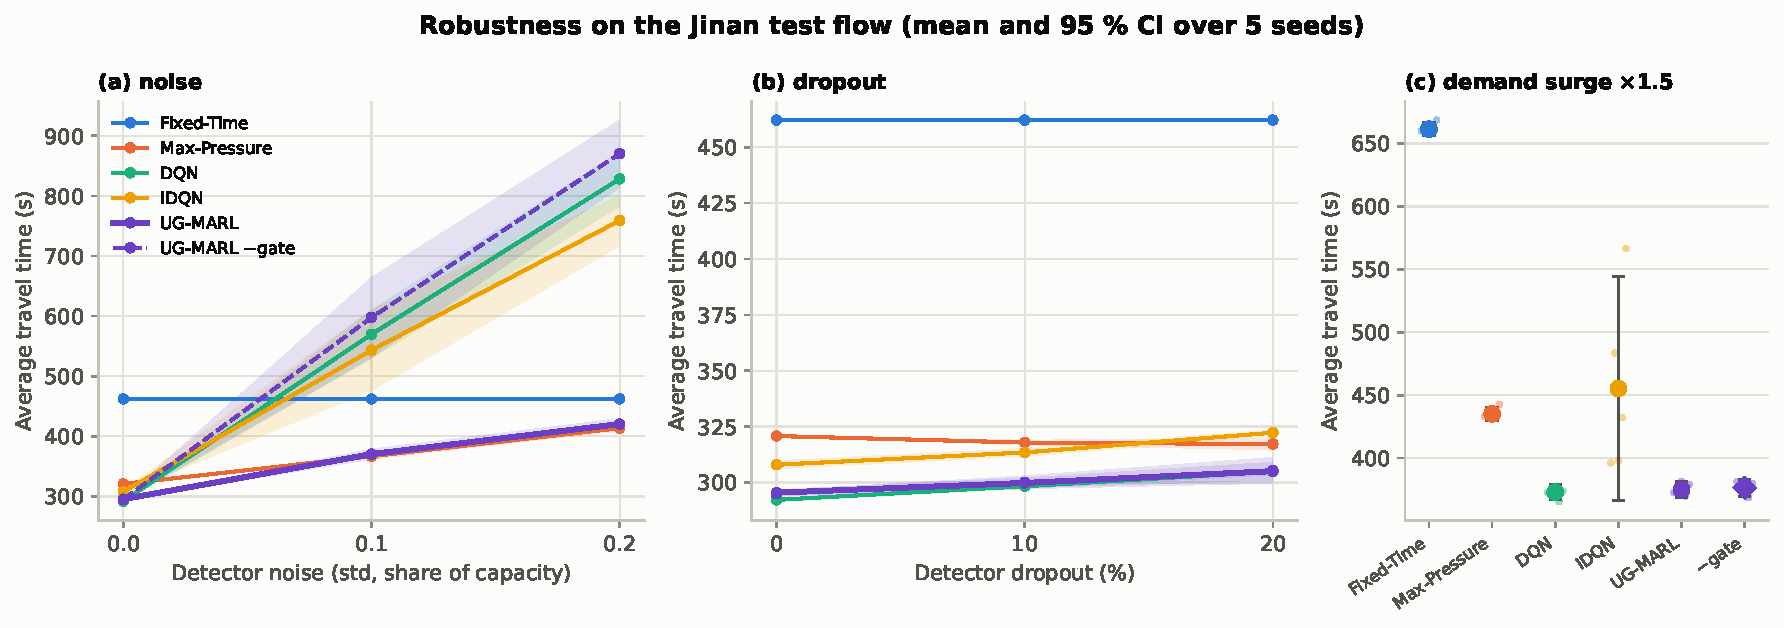
\includegraphics[width=\textwidth]{robustness_degradation.pdf}
\caption[Robustness to detector noise, dropout and demand surge]{Robustness on the Jinan test flow (mean and 95\,\% CI over 5 seeds). (a) Under
detector noise the ungated learned controllers lose 450--575\,s, while \ugmarl{} follows
Max-Pressure. (b) Dropout costs every controller less than 15\,s. (c) Under the demand surge
\ugmarl{} stays with DQN; IDQN becomes unstable across seeds.}
\label{fig:robust}
\end{figure}

\Cref{fig:robust} plots travel time against the three kinds of disturbance. The curves for
\ugmarl{} with and without the gate start at the same point and part as soon as noise is
added. Without the gate the model collapses under noise, and with it the model loses only as
much as Max-Pressure does. Dropout hardly matters, because a lost reading is set to zero and
looks like an empty lane, a state the agents saw in training.

\begin{figure}[t]
\centering
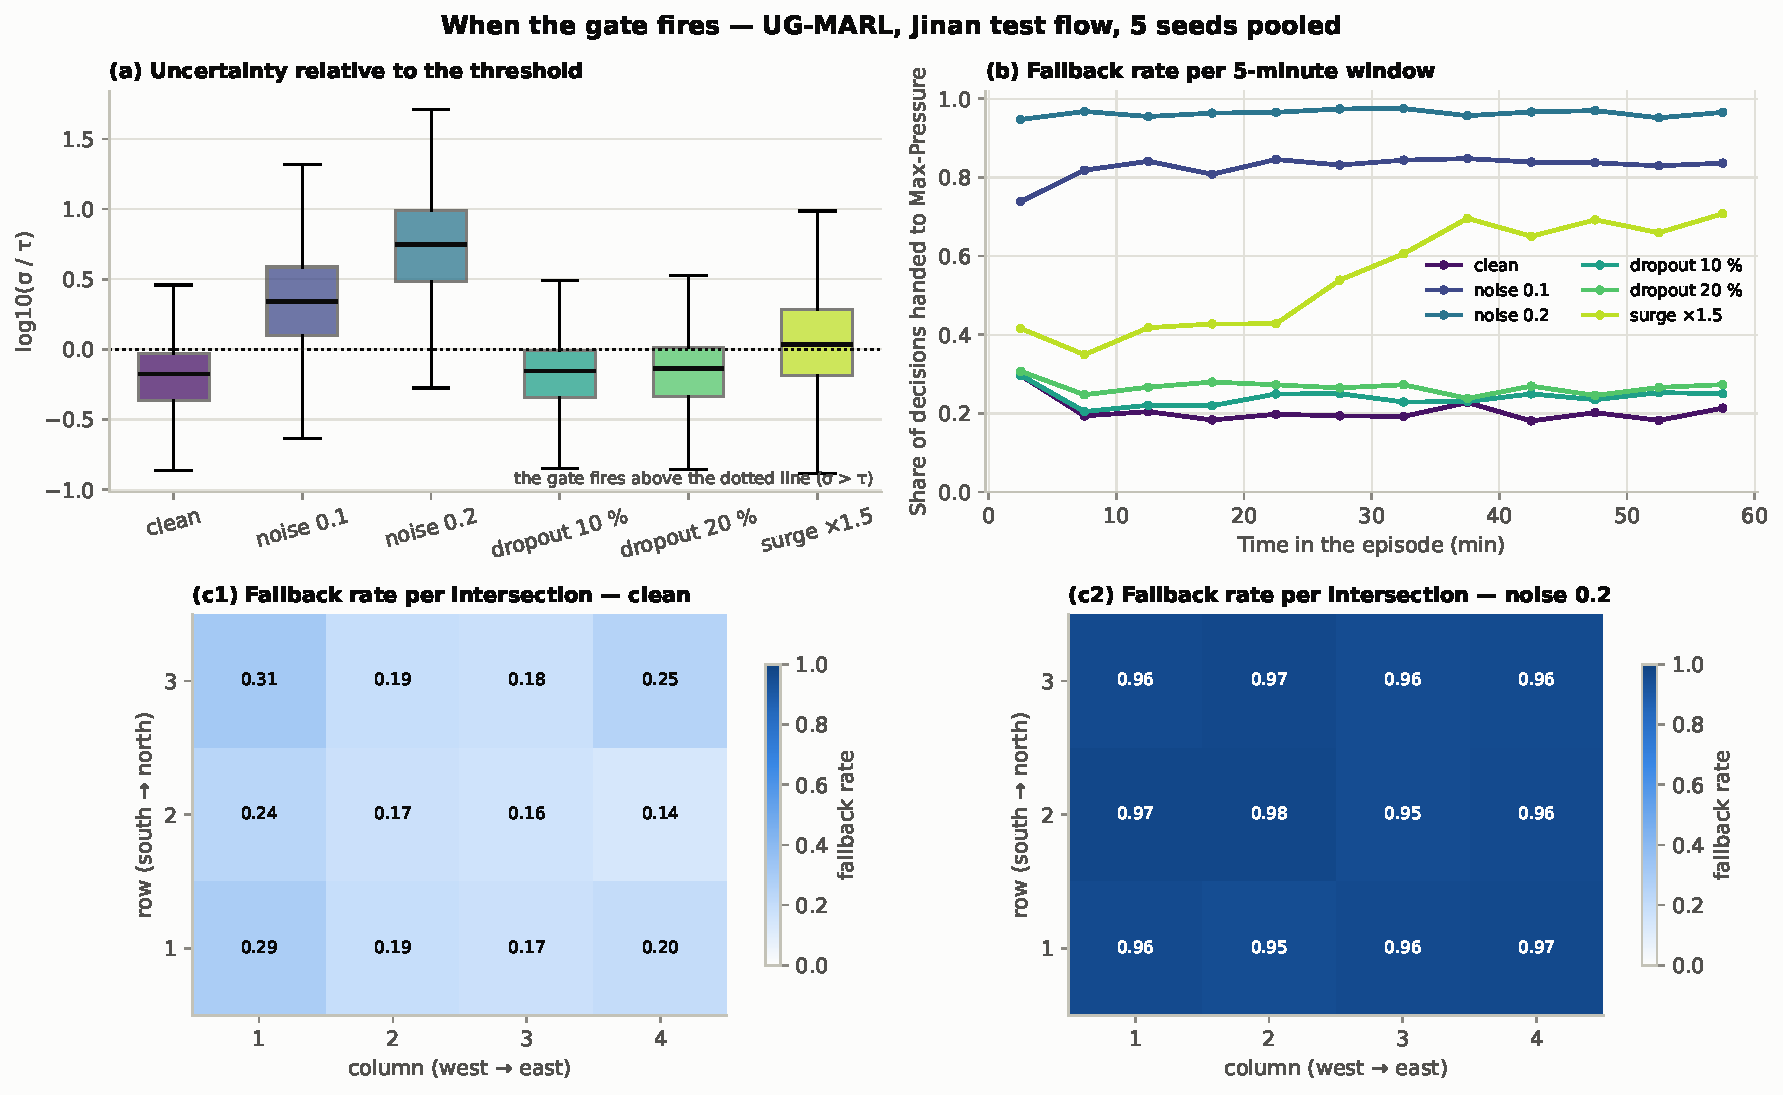
\includegraphics[width=0.68\textwidth]{gate_firing.pdf}
\caption[When and where the uncertainty gate fires]{When the gate fires (\ugmarl{}, Jinan test flow, 5 seeds pooled). (a) $\sigma$
relative to the threshold: the median is below $\tau$ on clean data and under dropout,
about $2\tau$ at noise 0.1 and $6\tau$ at noise 0.2. (b) Fallback rate over the hour: constant
except under the surge, where it rises from about 40 to 70\,\%. (c) Fallback rate per
intersection: 14--31\,\% on clean data, 95--98\,\% at noise 0.2.}
\label{fig:gate}
\end{figure}

\Cref{fig:gate} explains the pattern. The uncertainty $\sigma$ of \cref{eq:sigma} goes up
with detector noise, and the gate passes \res{fb}{ugmarl}{noise0.1}\,\% of decisions to
Max-Pressure at noise 0.1 and \res{fb}{ugmarl}{noise0.2}\,\% at noise 0.2, compared with
\res{fb}{ugmarl}{clean}\,\% on clean data. Dropout leaves it almost unchanged
(\res{fb}{ugmarl}{drop0.1} and \res{fb}{ugmarl}{drop0.2}\,\%). The detectors are clean during
the surge, yet $\sigma$ grows with the queues, and the fallback rate climbs through the hour
to an average of \res{fb}{ugmarl}{surge1.5}\,\%. In short, $\sigma$ responds to any input that
looks unlike the training data, whatever caused it.

\section{Discussion of Findings}
\label{sec:discussion}

\subsection{Ablation}
\begin{table}[t]
\centering\footnotesize
\setlength{\tabcolsep}{2.6pt}
\caption[Ablation of gate, attention and ensemble]{Ablation on the Jinan test flow (5 seeds). Travel time in seconds for three
conditions; $\Delta$ = difference to the full model on clean data; maximum wait in seconds;
FB = fallback rate on clean data.}
\label{tab:ablation}
% Generated by scripts/report_tables.py from docs/results/*.csv -- do not edit.
\begin{tabular}{lrrrrrrrr}
\toprule
Variant & Clean (s) & $\Delta$ (s) & Noise 0.2 (s) & Surge (s) & Max wait, clean & Max wait, noise 0.2 & FB (\%) & Params \\
\midrule
UG-MARL (full) & 295.4 $\pm$ 1.1 & -- & 420.5 $\pm$ 7.4 & 375.0 $\pm$ 4.9 & 896 $\pm$ 169 & 1493 $\pm$ 220 & 21 & 157\,720 \\
UG-MARL $-$gate & 295.0 $\pm$ 1.0 & $-$0.4 & 870.2 $\pm$ 45.0 & 376.4 $\pm$ 5.4 & 910 $\pm$ 190 & 3306 $\pm$ 323 & 0 & 157\,720 \\
UG-MARL $-$attention & 294.2 $\pm$ 1.1 & $-$1.2 & 419.3 $\pm$ 3.1 & 376.3 $\pm$ 2.8 & 876 $\pm$ 120 & 1410 $\pm$ 202 & 21 & 59\,032 \\
UG-MARL $-$ensemble & 297.3 $\pm$ 1.5 & $+$1.9 & 864.9 $\pm$ 134.8 & 395.1 $\pm$ 40.1 & 740 $\pm$ 238 & 3279 $\pm$ 259 & 0 & 89\,864 \\
\bottomrule
\end{tabular}

\end{table}

\Cref{tab:ablation} takes the three components out one at a time. Removing the
\emph{gate} changes nothing measurable on clean data (paired difference $0.4\pm0.9$\,s) and
costs 450\,s at noise 0.2. Without the \emph{ensemble} ($K=1$) there is no uncertainty
estimate and hence no gate, and the model fails under noise just like the other ungated
learners; on clean data it is 1.9\,s behind the full model, with overlapping intervals.
Without \emph{attention}, the model reaches \res{tt}{ugmarl-noattn}{clean}\,s against
\res{tt}{ugmarl}{clean}\,s for the full model, with overlapping intervals and 63\,\% fewer
parameters. \textbf{H3 is not supported}. Neighbour attention did not lower travel time in
any of the six conditions or on Hangzhou.

\subsection{Generalisation}
\begin{table}[t]
\centering\footnotesize
\setlength{\tabcolsep}{3.6pt}
\caption[Zero-shot generalisation to Hangzhou]{Zero-shot evaluation on Hangzhou ($4\times4$, three flows, 5 seeds): average
travel time in seconds. Models were trained on the Jinan training flow and thresholds come
from Jinan validation. ``All flows'' averages the flows per seed; maximum wait and fallback
rate (FB) are over all flows. Bold: lowest travel time.}
\label{tab:heldout}
% Generated by scripts/report_tables.py from docs/results/*.csv -- do not edit.
\begin{tabular}{lrrrrcrr}
\toprule
Model & Flow A & Flow B & Flow C & All flows (s) & 95\,\% CI & Max wait (s) & FB (\%) \\
\midrule
Fixed-Time & 590.5 & 841.7 & 570.2 & 667.5 & -- & 1756 & 0 \\
Max-Pressure & 360.7 & 500.0 & 434.7 & 431.8 & -- & 2734 & 0 \\
\midrule
DQN (shared) & 343.4 $\pm$ 2.1 & 478.7 $\pm$ 22.7 & 409.1 $\pm$ 4.9 & 410.4 $\pm$ 7.1 & [401.6, 419.3] & 1660 $\pm$ 272 & 0 \\
IDQN & \multicolumn{7}{c}{not transferable (one network per Jinan intersection)} \\
\midrule
UG-MARL (proposed) & 347.3 $\pm$ 3.5 & 466.4 $\pm$ 8.5 & 416.3 $\pm$ 2.6 & 410.0 $\pm$ 2.9 & [406.4, 413.6] & 2262 $\pm$ 206 & 34 \\
UG-MARL $-$gate & 348.9 $\pm$ 4.3 & 491.7 $\pm$ 35.6 & 419.8 $\pm$ 10.1 & 420.1 $\pm$ 14.6 & [402.0, 438.2] & 1939 $\pm$ 375 & 0 \\
UG-MARL $-$attention & 341.5 $\pm$ 0.7 & 460.2 $\pm$ 5.1 & 409.6 $\pm$ 1.9 & \textbf{403.8 $\pm$ 1.2} & [402.3, 405.2] & 2146 $\pm$ 153 & 37 \\
UG-MARL $-$ensemble & 351.7 $\pm$ 2.9 & 493.7 $\pm$ 39.2 & 425.7 $\pm$ 8.9 & 423.7 $\pm$ 14.9 & [405.2, 442.2] & 1696 $\pm$ 237 & 0 \\
\bottomrule
\end{tabular}

\end{table}

\Cref{tab:heldout} shows the zero-shot results on a city and a grid size that played no
part in training or tuning. The ranking is the same as on Jinan: learned controllers first,
then Max-Pressure, then Fixed-Time. \ugmarl{} (\res{tt}{ugmarl}{hz-all}\,s) is level with DQN
(\res{tt}{dqn}{hz-all}\,s) and 22\,s ahead of Max-Pressure. Its gate fires more often here
than on Jinan (\res{fb}{ugmarl}{hz-all}\,\% against \res{fb}{ugmarl}{clean}\,\%), and it
removes most of the spread between seeds that the ungated model shows
($\pm$\res{ttsd}{ugmarl}{hz-all} against $\pm$\res{ttsd}{ugmarl-nogate}{hz-all}\,s). IDQN
cannot be moved to Hangzhou at all, since it keeps one network for each Jinan intersection.

\subsection{Error analysis}
The saved logs were split by intersection, by 10-minute window and by route.
\begin{itemize}
\item \emph{Where \ugmarl{} wins.} Compared with Max-Pressure on clean data, vehicles wait
17--40\,\% less at each of the 12 intersections. The gain grows with route length, from 12\,s
for trips through one intersection to 37\,s for trips through four or more.
\item \emph{Where it loses.} The 3.2\,s deficit to DQN is spread out. Waiting is higher at
every intersection (by up to 12\,\%), in every time window and for every route length. The
gate is not to blame, because the same checkpoints without it are level with the gated model.
All four \ugmarl{} variants trail DQN, so the gap comes either from the network family or
from its learning settings, which were tuned for DQN and reused. The available runs cannot tell
these two apart.
\item \emph{A failure the metrics hide.} At noise 0.2 the ungated learned controllers keep
584--795 of the 5494 vehicles (11--14\,\%) out of the network for the whole hour, because the
entry roads stay jammed. \ugmarl{} and Max-Pressure keep none out. The waiting-time metrics
only count waiting \emph{inside} the network, so the maximum wait of about 3300\,s reported
for these models understates how badly they do.
\item \emph{What the gate costs under a surge.} During the surge the gate leaves travel time
unchanged (\res{tt}{ugmarl}{surge1.5} against \res{tt}{ugmarl-nogate}{surge1.5}\,s) but pushes
the maximum wait up to \res{maxw}{ugmarl}{surge1.5}\,s, compared with
\res{maxw}{ugmarl-nogate}{surge1.5}\,s without the gate and \res{maxw}{dqn}{surge1.5}\,s for
DQN. Max-Pressure alone reaches \res{maxw}{max_pressure}{surge1.5}\,s. Once the gate hands it
most of the decisions, \ugmarl{} picks up its habit of leaving single vehicles waiting a long
time. The most congested Hangzhou flow shows the same thing.
\item \emph{Stability of decisions.} \ugmarl{} switches back to the previous phase after one
interval in 21.5\,\% of its decisions, against 20.2\,\% for DQN and 20.3\,\% for
Max-Pressure, so the gate does not add switching.
\end{itemize}

\subsection{Explainability}
For each decision the system logs $\sigma$, $\tau$, whether the gate fired, the learned
phase, the Max-Pressure phase and the attention weights. These are associations, and two
checks on validation data show how far they can be read. The first is that $\sigma$ has almost
no correlation with the temporal-difference error (Spearman $\rho\approx0.03$). It flags
unfamiliar inputs and says little about whether an action is wrong. The second check swaps
out one neighbour's observation. Swapping the neighbour with the highest attention weight
moves the Q-value more than swapping the one with the lowest (0.0061 against 0.0022, paired
interval $[0.0011, 0.0066]$), so the weights do rank the neighbours' influence. Doing the same
to the intersection's own observation moves Q by 0.0415, about seven times as much, and the own
slot gets a mean weight of 0.82. Decisions are therefore made almost entirely from local
information, which fits the H3 result. One likely reason is that the movement pressures in
\cref{eq:state} already include the downstream lanes that a neighbour would report.

\subsection{Threshold and cost}
A validation sweep run after the final evaluation shows that the exact threshold matters
little. Every percentile from 50 to 90 lands within 5\,s of the chosen $p^\star=80$. $p=70$
would have been 1.5\,s better, so the bottom of the original grid was binding, but the choice
was left as it was. One joint decision for all 12 intersections takes 0.81\,ms with \ugmarl{},
0.22\,ms with DQN and 0.14\,ms with Max-Pressure on a single CPU thread, far inside the 15\,s
decision interval.
